\documentclass[xcolor=table]{beamer}
\usepackage[utf8]{inputenc}
\usepackage[francais]{babel}
%\usetheme{Boadilla}
%\usecolortheme{rose}
%\usecolortheme{crane}
\usefonttheme{structuresmallcapsserif}
\setbeamertemplate{navigation symbols}{}

\definecolor{Main}{rgb}{0.74, 0.13, 0.19}
\definecolor{Accent1}{rgb}{0.76,0.36,0.13}
\definecolor{Accent2}{rgb}{0.54,0.1,0.4}

\usecolortheme{rose}
%\useinnertheme[shadow]{circles}
\usecolortheme{whale}
%\useoutertheme{infolines}

\usecolortheme[named=Accent1]{structure}

\setbeamercolor{alerted text}{fg=Accent2}
%\setbeamercolor{palette primary}{fg=white}
%\setbeamercolor{palette secondary}{bg=Accent1}
%\setbeamercolor{palette tertiary}{bg=Accent2,fg=white}


\setbeamerfont{page number in head/foot}{size=\large}
\setbeamercolor{page number in head/foot}{fg=Main}
% page/total
%\setbeamertemplate{footline}[frame number]
% pas de total
\setbeamertemplate{footline}{%
    	\hfill%
	\usebeamercolor[fg]{page number in head/foot}%
	\usebeamerfont{page number in head/foot}%
	\insertframenumber\kern1em\vskip2pt%
}

\setbeamersize{text margin left=1em}
\setbeamersize{text margin right=1em}

%font
\usepackage[T1]{fontenc}
\usepackage[oldstylenums]{kpfonts}


%proper math and math symbols
%\usepackage{amsmath}
\usepackage{amssymb}

\usepackage{datenumber,fp}

\usepackage{siunitx}

\usepackage{tabu}
\usepackage{multirow}
\usepackage{booktabs}

% Allow the usage of graphics (.jpg, .png, etc.) in the document
\usepackage{graphicx}
\usepackage{tikz}
\usetikzlibrary{arrows,shapes,backgrounds, calc, positioning, topaths,chains, intersections, decorations.markings, shapes.geometric, matrix,patterns,mindmap}
%\usetikzlibrary{positioning, patterns,topaths,chains,matrix}

\usepackage{pgfplots}
\usepgfplotslibrary{groupplots}
\usepgfplotslibrary{external}



%beamer related package

\usepackage{todonotes}
\presetkeys{todonotes}{inline}{}


%bibliography
\usepackage[style=authoryear-comp, language=british,eprint=false, url=false, doi=false, sortcites=true, sorting=none, isbn=false, firstinits=true,maxcitenames=6]{biblatex}
%minimal citations
\AtEveryCitekey{%
	\clearfield{title}
	\clearfield{pages}
	\clearfield{volume}
	\clearfield{number}
	\clearfield{month}}
\newcommand{\myfullcite}[1]{{\scriptsize\fullcite{#1}}}
\renewbibmacro{in:}{%
  \ifentrytype{article}{}{%
  \printtext{\bibstring{in}\intitlepunct}}}
%\bibliography{biblio}


\newcolumntype{P}[1]{>{\raggedright}p{#1}}


\begin{document}
\tikzset{every mark/.append style={scale=0.8}}
\pgfplotsset{compat=1.3, every axis/.append style={footnotesize}}

\begin{frame}{Looking for a yield stress}

\begin{columns}
\column{0.5\textwidth}

\begin{block}{Upside-down test}
\begin{tabu}{b{3em}X[b]}
\begin{tikzpicture}
\fill[Accent1!50] (0,1em) rectangle (1em, 4em);
\draw (0,0) -- (0,4em) -- (1em, 4em) -- (1em,0);
\draw[->, Main] (0.5em,1.5em) -- +(0,-1em) node[below] {$\sigma$};
\draw[<->] (1.25em, 1em) -- +(0,3em) node[midway, right] {$h$};
\end{tikzpicture} &
Flows if $\alert{\sigma_Y} < \sigma = \rho g h$\linebreak
Actually, more complicated because surface tension
\end{tabu}
\end{block}

\structure{Cone-plate geometry}

\begin{center}
\begin{tikzpicture}
%sample
\fill[Accent1!50] (3em,0) arc (0:10:3em)  -- (170:3em) arc (170:180:3em) --cycle;
%cone
\fill[gray] (10:0.1em) -- (10:3em) -- (170:3em) -- (170:0.1em)  -- cycle;
\filldraw[gray]  (10:3em) +(0,0.1em) rectangle (170:3em);
%tige
\fill[gray] +(-0.5em,0.5em) rectangle +(0.5em, 3em);
\draw[->, Accent2] (-1em, 3em) arc (-180:0:1em and 0.5em) node[below right] {$\dot{\gamma}$};
%plate
\fill[gray] (-4em,0) rectangle (4em, -1em);
\end{tikzpicture}
\end{center}

\begin{itemize}
\item Can't spin too fast
\item Can't use ultrasound velocimetry
\end{itemize}


\column{0.5\textwidth}
Carbopol microgel\\
\textit{Divoux et al. 2012}
\includegraphics[width=\textwidth]{Divoux_Herschel–Bulkley.png}

\begin{block}{Herschel-Bulkley}
\[ \sigma = \alert{\sigma_Y} + K \dot{\gamma}^n \]
\end{block}
\end{columns}
\end{frame}

\begin{frame}{Herschel-Bulkley fluid?}
\[ \sigma = \alert{\sigma_Y} + K \dot{\gamma}^n \]
\begin{columns}
\column{0.5\textwidth}
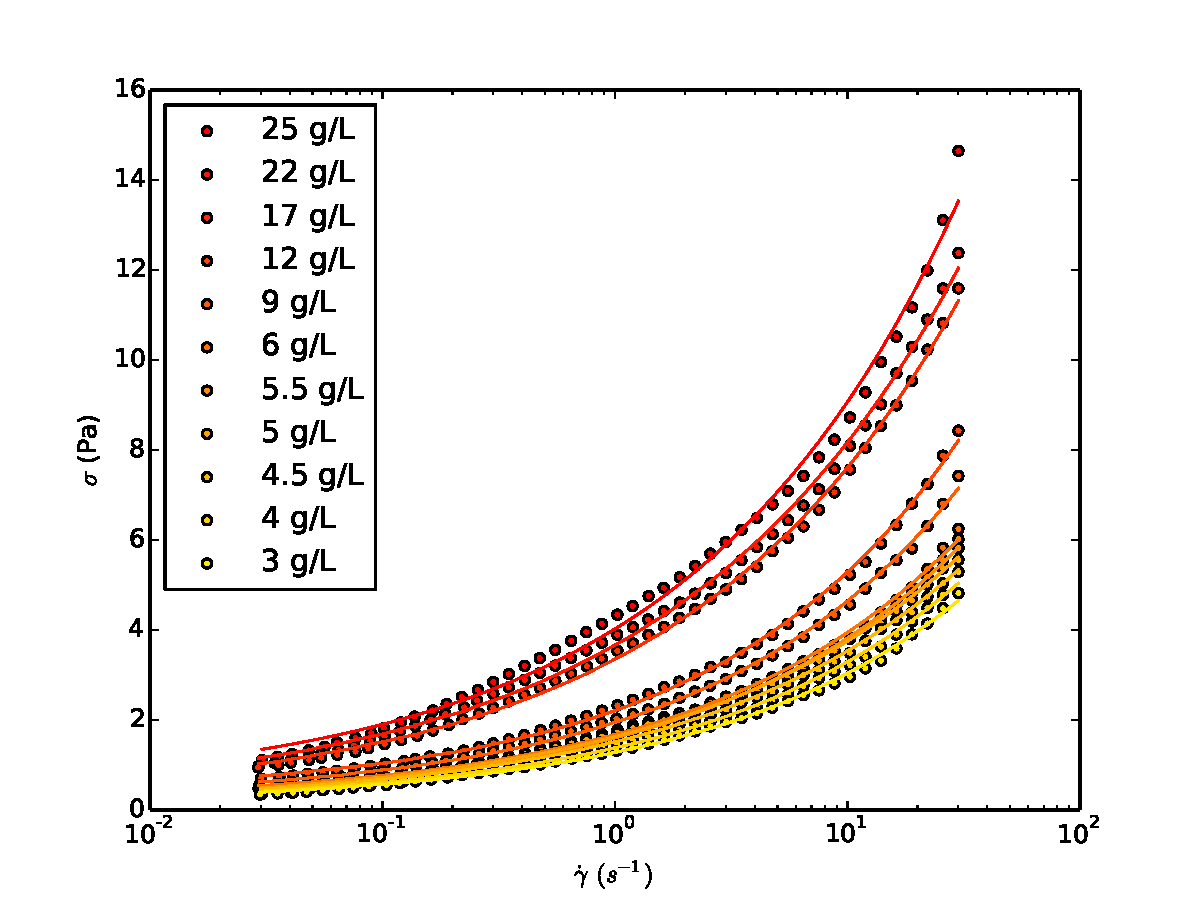
\includegraphics[width=\textwidth]{HershelBuckley_only_r1}
\column{0.5\textwidth}
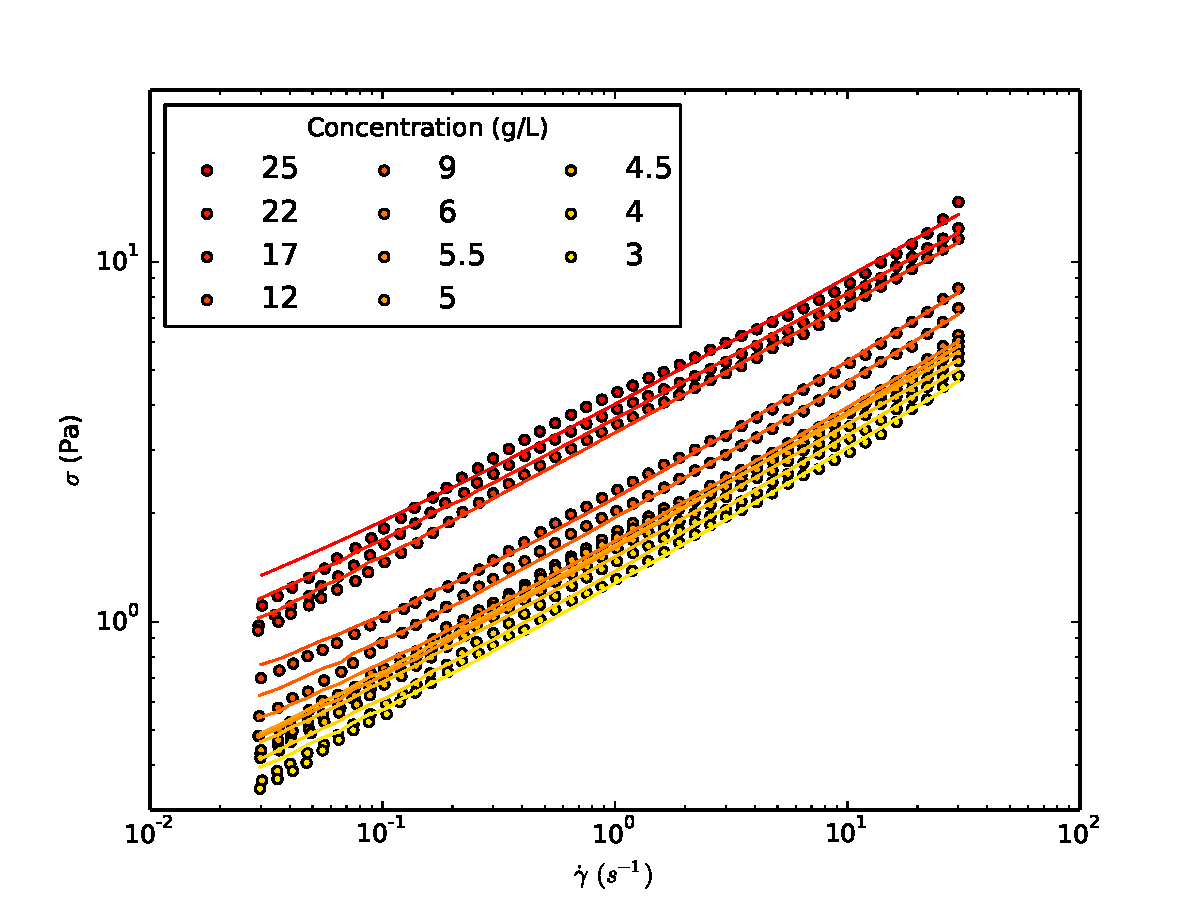
\includegraphics[width=\textwidth]{HershelBuckley_loglog_r1}
\end{columns}
\end{frame}

\begin{frame}{Or power-law fluid?}
\[ \sigma = K \dot{\gamma}^n\]
\begin{columns}
\column{0.5\textwidth}
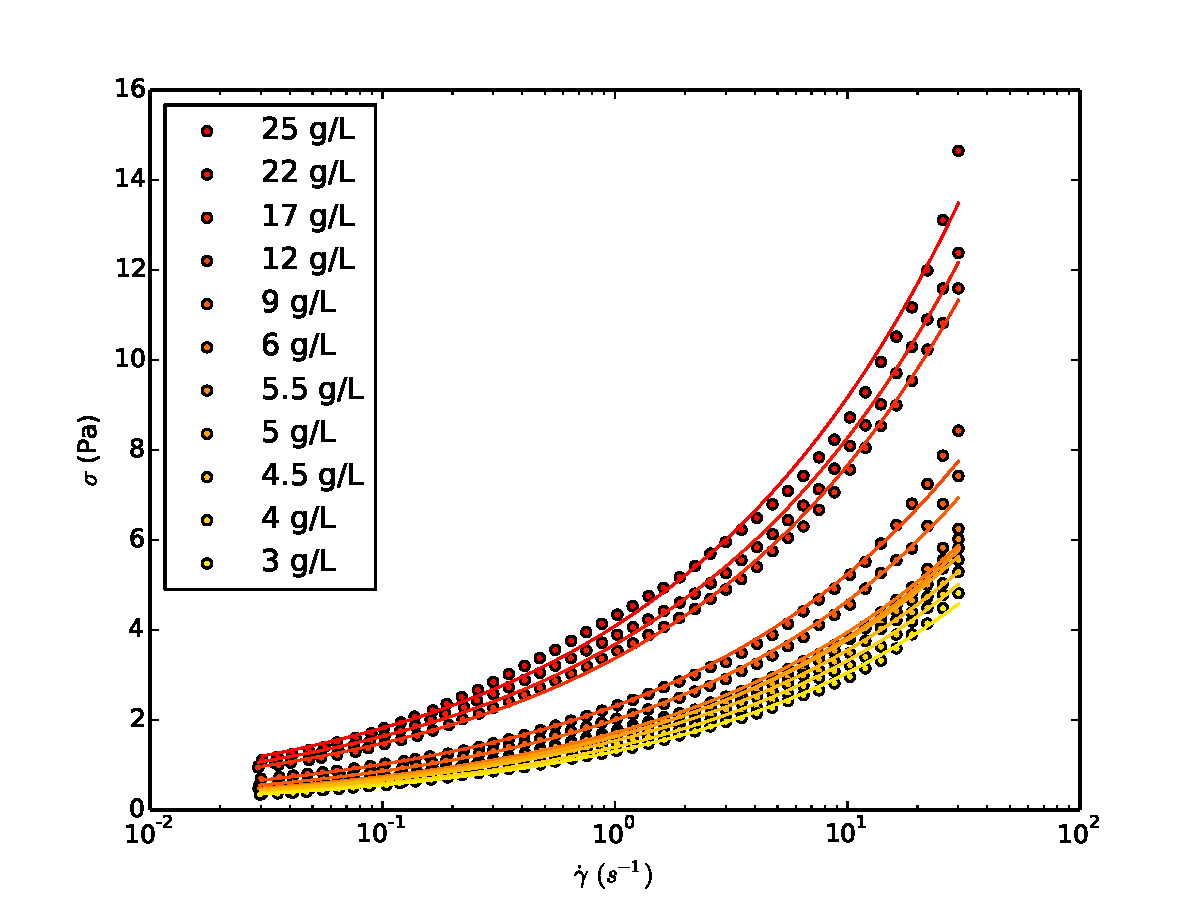
\includegraphics[width=\textwidth]{Power-law_logx_r1}
\column{0.5\textwidth}
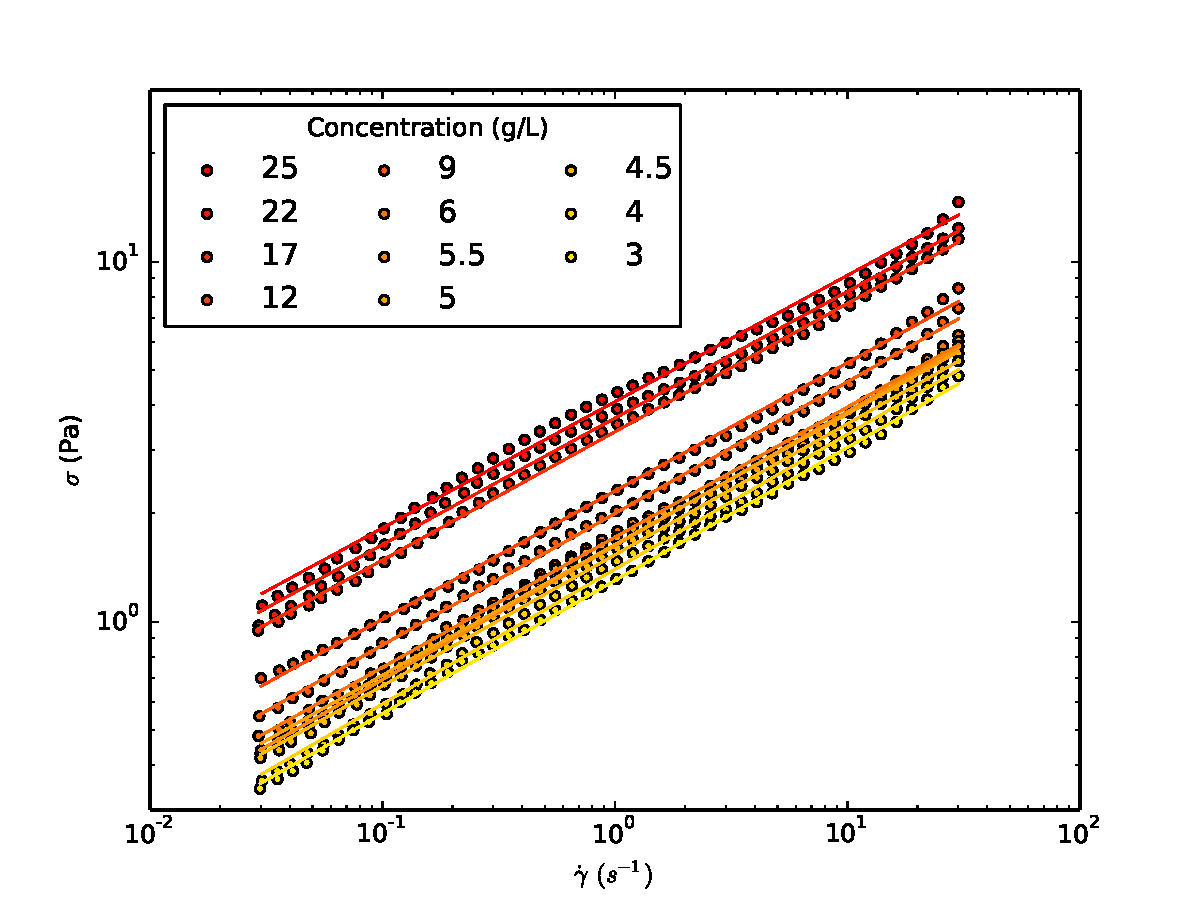
\includegraphics[width=\textwidth]{Power-law_r1}
\end{columns}
\end{frame}

\begin{frame}{Or Herschel-Bulkley with slip at the wall?}
\[ \sigma = \alert{\sigma_Y} + K \dot{\gamma}^n  \qquad\text{for}\quad\dot{\gamma}>\SI{1}{\per\second}\]
\begin{columns}
\column{0.5\textwidth}
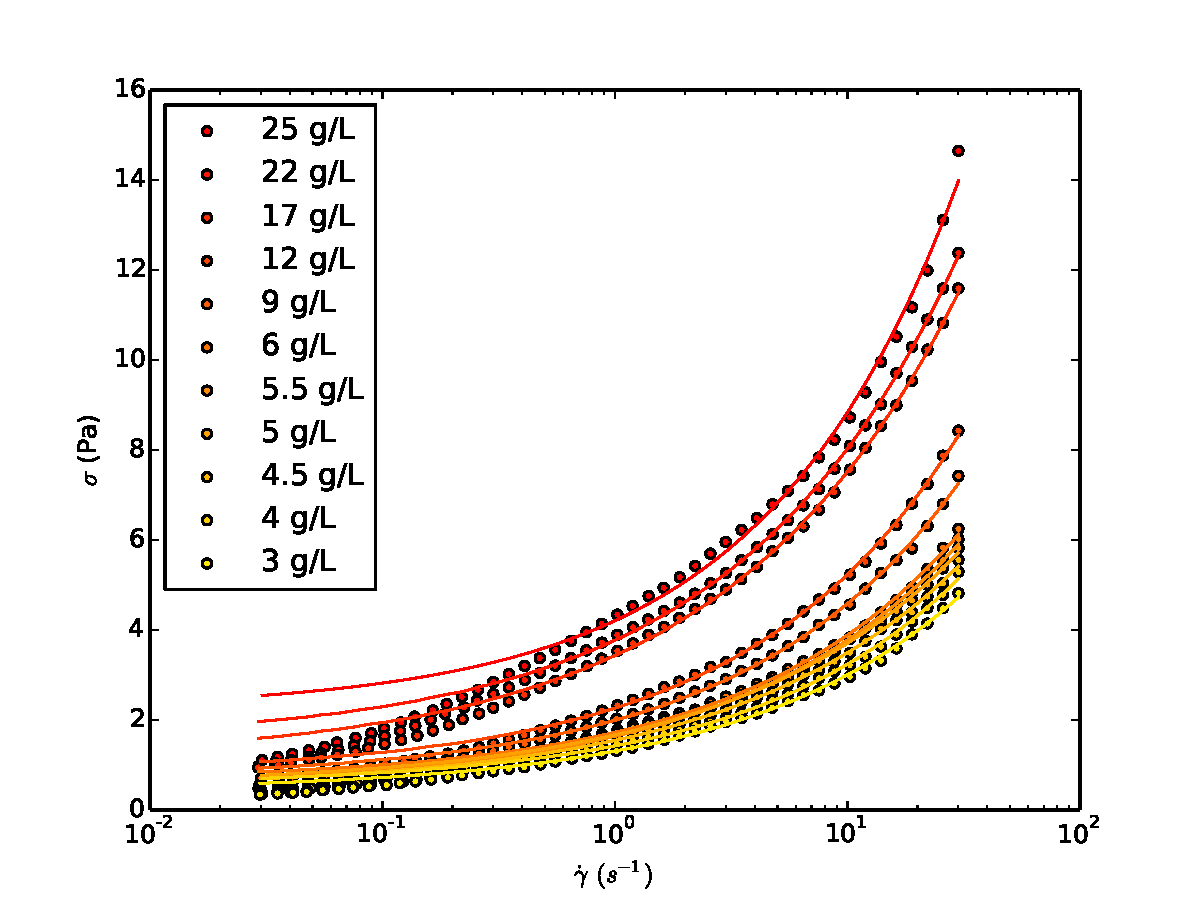
\includegraphics[width=\textwidth]{HershelBuckley_r1}
\column{0.5\textwidth}
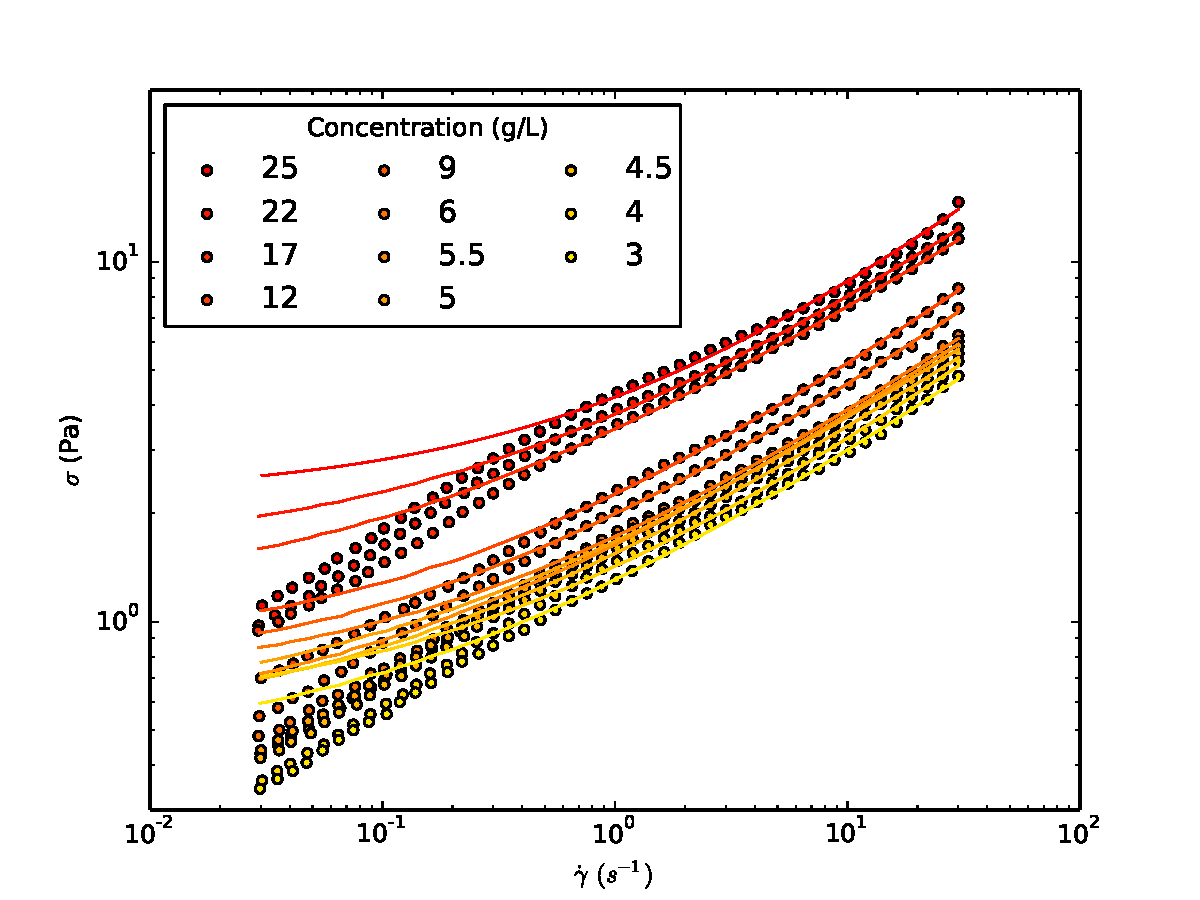
\includegraphics[width=\textwidth]{HershelBuckley_slip_loglog_r1}
\end{columns}
\end{frame}

\begin{frame}{Yield stress vs concentration}
\begin{center}
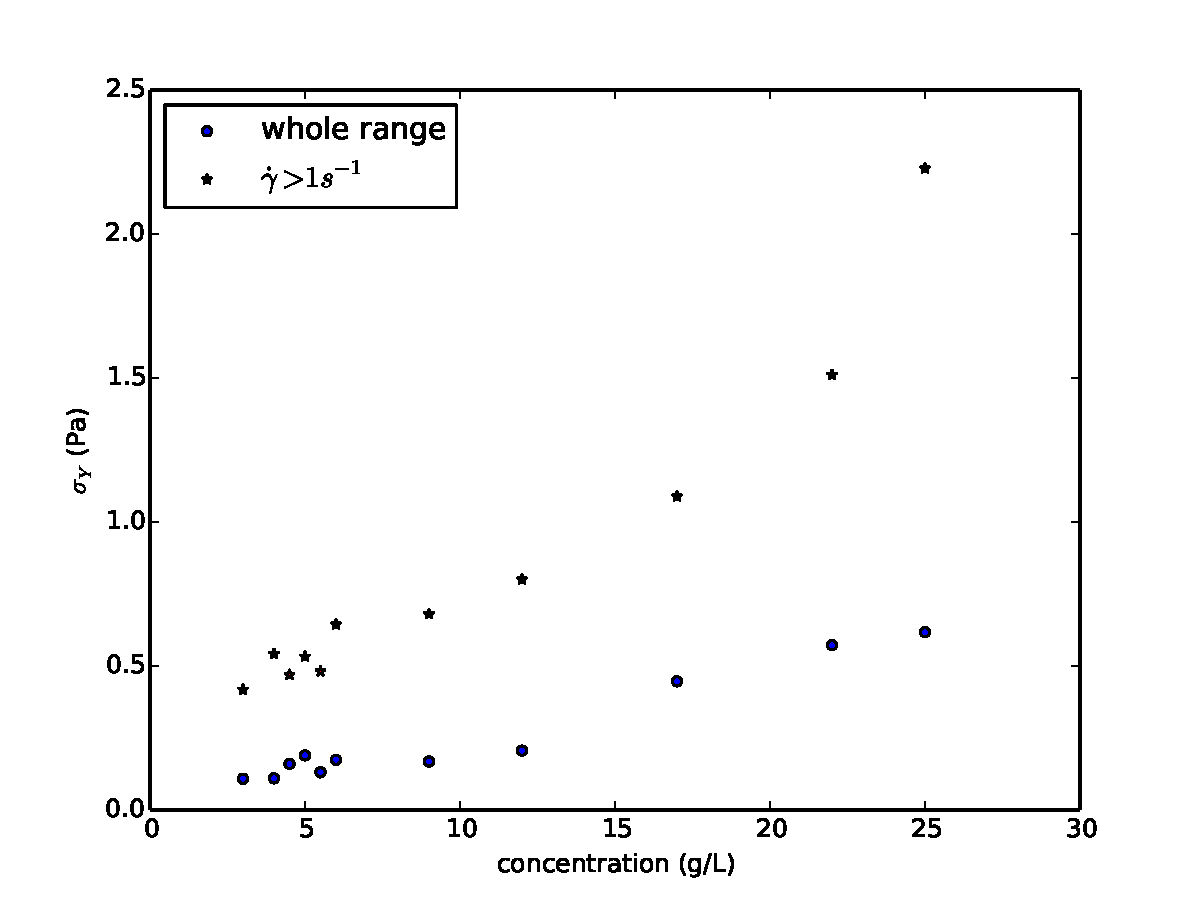
\includegraphics[height=\textheight-3\baselineskip]{yield_stress_r1}
\end{center}
\end{frame}

\begin{frame}{Time to use Couette geometry}
\begin{columns}
\column{0.35\textwidth}
\begin{tikzpicture}
	\draw circle[x radius=0.5\textwidth, y radius=0.1\textwidth] +(0,-5\baselineskip) circle;
	\fill (0,0.015\textwidth) circle [x radius=0.4\textwidth, y radius=0.08\textwidth];
	\draw[->, white, x radius=0.2\textwidth, y radius=0.05\textwidth]  (0,0.03\textwidth) +(90:0.05\textwidth) arc[start angle=90, end angle=270] node[right=1mm, font=\scriptsize] {$\dot{\gamma}$};
	\draw (0.5\textwidth,0) -- +(0,-5\baselineskip) arc[x radius=0.5\textwidth, y radius=0.1\textwidth, start angle=0, end angle=-180] -- +(0,5\baselineskip);
	\draw[dotted] (0.4\textwidth,0.015\textwidth) -- +(0,-5\baselineskip) arc[x radius=0.4\textwidth, y radius=0.09\textwidth, start angle=0, end angle=-180] -- +(0,5\baselineskip);
\end{tikzpicture}

\column{0.65\textwidth}
\begin{itemize}
\item Higher shear rates
\item Less evaporation
\item Possible to use Ultrasound velocimetry
\begin{itemize}
\item To quantify wall slip
\item To observe instabilities at high shear rate
\end{itemize}
\item[But] much more sample needed (\SI{20}{\milli\litre})
\end{itemize}
\end{columns}
\end{frame}

\end{document}

